% This file was created by tikzplotlib v0.8.2.
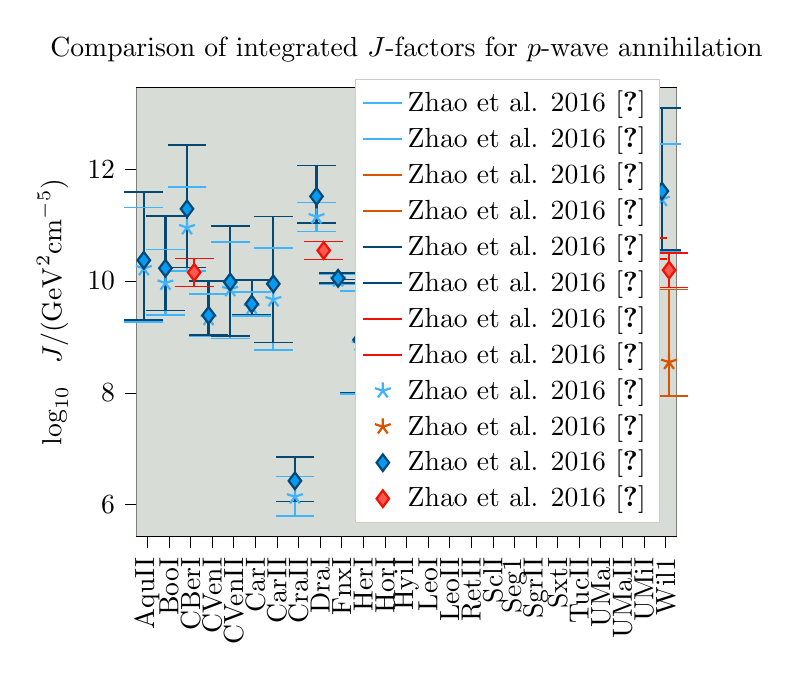
\begin{tikzpicture}

\definecolor{color0}{rgb}{0.250850460666195,0.707122608079376,0.981502480510276}
\definecolor{color1}{rgb}{0.844117647058824,0.335069600359228,0}
\definecolor{color2}{rgb}{0.0111977321048902,0.287408457358847,0.453508150248051}
\definecolor{color3}{rgb}{0.936880370125579,0.069596827495043,0.0160608063450098}
\definecolor{color4}{rgb}{0.500566973777463,0.804748405386251,0.987668320340184}
\definecolor{color5}{rgb}{1,0.535294117647059,0.229411764705882}
\definecolor{color6}{rgb}{0.847058823529412,0.862745098039216,0.83921568627451}
\definecolor{color7}{rgb}{0.0235294117647059,0.603921568627451,0.952941176470588}
\definecolor{color8}{rgb}{0.988235294117647,0.352941176470588,0.313725490196078}

\begin{axis}[
legend cell align={left},
legend style={at={(0.97,0.03)}, anchor=south east, draw=white!80.0!black},
tick align=outside,
tick pos=left,
title={Comparison of integrated $J$-factors for $p$-wave annihilation},
x grid style={white!69.01960784313725!black},
xmin=0.5, xmax=25.5,
xtick style={color=black},
xtick={1,2,3,4,5,6,7,8,9,10,11,12,13,14,15,16,17,18,19,20,21,22,23,24,25},
xticklabel style = {rotate=90.0},
xticklabels={~AquII,~~BooI,~CBerI,~CVenI,CVenII,~~CarI,~CarII,~CraII,~~DraI,~~FnxI,~~HerI,~~HorI,~~HyiI,~~LeoI,~LeoII,~RetII,~~SclI,~~Seg1,~SgrII,~~SxtI,~TucII,~~UMaI,~UMaII,~~UMiI,~~Wil1},
y grid style={white!50.19607843137255!black},
ylabel={\(\displaystyle \log_{10}\,\,\,\,J/(\mathrm{GeV}^2\mathrm{cm}^{-5})\)},
ymajorgrids,
ymin=5.43643790202566, ymax=13.4520585682647,
yminorgrids,
ytick style={color=black}
]
\addplot [line width=17.6pt, color6, forget plot]
table {%
0 5.43643790202566
0 13.4520585682647
};
\addplot [line width=17.6pt, color6, forget plot]
table {%
2 5.43643790202566
2 13.4520585682647
};
\addplot [line width=17.6pt, color6, forget plot]
table {%
4 5.43643790202566
4 13.4520585682647
};
\addplot [line width=17.6pt, color6, forget plot]
table {%
6 5.43643790202566
6 13.4520585682647
};
\addplot [line width=17.6pt, color6, forget plot]
table {%
8 5.43643790202566
8 13.4520585682647
};
\addplot [line width=17.6pt, color6, forget plot]
table {%
10 5.43643790202566
10 13.4520585682647
};
\addplot [line width=17.6pt, color6, forget plot]
table {%
12 5.43643790202566
12 13.4520585682647
};
\addplot [line width=17.6pt, color6, forget plot]
table {%
14 5.43643790202566
14 13.4520585682647
};
\addplot [line width=17.6pt, color6, forget plot]
table {%
16 5.43643790202566
16 13.4520585682647
};
\addplot [line width=17.6pt, color6, forget plot]
table {%
18 5.43643790202566
18 13.4520585682647
};
\addplot [line width=17.6pt, color6, forget plot]
table {%
20 5.43643790202566
20 13.4520585682647
};
\addplot [line width=17.6pt, color6, forget plot]
table {%
22 5.43643790202566
22 13.4520585682647
};
\addplot [line width=17.6pt, color6, forget plot]
table {%
24 5.43643790202566
24 13.4520585682647
};
\addplot [line width=17.6pt, color6, forget plot]
table {%
26 5.43643790202566
26 13.4520585682647
};
\addplot [line width=17.6pt, color6, forget plot]
table {%
0 5.43643790202566
0 13.4520585682647
};
\addplot [line width=17.6pt, color6, forget plot]
table {%
2 5.43643790202566
2 13.4520585682647
};
\addplot [line width=17.6pt, color6, forget plot]
table {%
4 5.43643790202566
4 13.4520585682647
};
\addplot [line width=17.6pt, color6, forget plot]
table {%
6 5.43643790202566
6 13.4520585682647
};
\addplot [line width=17.6pt, color6, forget plot]
table {%
8 5.43643790202566
8 13.4520585682647
};
\addplot [line width=17.6pt, color6, forget plot]
table {%
10 5.43643790202566
10 13.4520585682647
};
\addplot [line width=17.6pt, color6, forget plot]
table {%
12 5.43643790202566
12 13.4520585682647
};
\addplot [line width=17.6pt, color6, forget plot]
table {%
14 5.43643790202566
14 13.4520585682647
};
\addplot [line width=17.6pt, color6, forget plot]
table {%
16 5.43643790202566
16 13.4520585682647
};
\addplot [line width=17.6pt, color6, forget plot]
table {%
18 5.43643790202566
18 13.4520585682647
};
\addplot [line width=17.6pt, color6, forget plot]
table {%
20 5.43643790202566
20 13.4520585682647
};
\addplot [line width=17.6pt, color6, forget plot]
table {%
22 5.43643790202566
22 13.4520585682647
};
\addplot [line width=17.6pt, color6, forget plot]
table {%
24 5.43643790202566
24 13.4520585682647
};
\addplot [line width=17.6pt, color6, forget plot]
table {%
26 5.43643790202566
26 13.4520585682647
};
\path [draw=color0, thick]
(axis cs:0.833333333333333,9.26103063784371)
--(axis cs:0.833333333333333,11.3131661596271);

\path [draw=color0, thick]
(axis cs:1.83333333333333,9.38839371042479)
--(axis cs:1.83333333333333,10.5644185723166);

\path [draw=color0, thick]
(axis cs:3.83333333333333,9.01815608310211)
--(axis cs:3.83333333333333,9.76638864010926);

\path [draw=color0, thick]
(axis cs:4.83333333333333,8.97028887193948)
--(axis cs:4.83333333333333,10.6938744616447);

\path [draw=color0, thick]
(axis cs:5.83333333333333,9.3736764619762)
--(axis cs:5.83333333333333,9.80044541591975);

\path [draw=color0, thick]
(axis cs:6.83333333333333,8.76892621794355)
--(axis cs:6.83333333333333,10.591979925665);

\path [draw=color0, thick]
(axis cs:2.83333333333333,10.1823445990016)
--(axis cs:2.83333333333333,11.6833657273993);

\path [draw=color0, thick]
(axis cs:7.83333333333333,5.80078429594561)
--(axis cs:7.83333333333333,6.50622111812952);

\path [draw=color0, thick]
(axis cs:8.83333333333333,10.8828709970361)
--(axis cs:8.83333333333333,11.4030948257365);

\path [draw=color0, thick]
(axis cs:9.83333333333333,9.93364833404171)
--(axis cs:9.83333333333333,10.1159848504708);

\path [draw=color0, thick]
(axis cs:10.8333333333333,7.98209341715927)
--(axis cs:10.8333333333333,9.82295625654854);

\path [draw=color0, thick]
(axis cs:11.8333333333333,10.158598682609)
--(axis cs:11.8333333333333,12.761106983693);

\path [draw=color0, thick]
(axis cs:12.8333333333333,9.47916908573022)
--(axis cs:12.8333333333333,10.8681048456269);

\path [draw=color0, thick]
(axis cs:13.8333333333333,9.51430778775519)
--(axis cs:13.8333333333333,10.238605824132);

\path [draw=color0, thick]
(axis cs:14.8333333333333,9.30775538828968)
--(axis cs:14.8333333333333,10.2232619485354);

\path [draw=color0, thick]
(axis cs:15.8333333333333,9.8365184246902)
--(axis cs:15.8333333333333,11.4402134334773);

\path [draw=color0, thick]
(axis cs:18.8333333333333,7.48136444868366)
--(axis cs:18.8333333333333,10.225375305854);

\path [draw=color0, thick]
(axis cs:16.8333333333333,10.4302157837854)
--(axis cs:16.8333333333333,10.6065575958899);

\path [draw=color0, thick]
(axis cs:17.8333333333333,9.54714398960339)
--(axis cs:17.8333333333333,11.4133652561043);

\path [draw=color0, thick]
(axis cs:19.8333333333333,9.31064127533647)
--(axis cs:19.8333333333333,9.60524129599008);

\path [draw=color0, thick]
(axis cs:20.8333333333333,10.0997178866913)
--(axis cs:20.8333333333333,11.7588667198827);

\path [draw=color0, thick]
(axis cs:21.8333333333333,9.68902026034909)
--(axis cs:21.8333333333333,10.7050058116999);

\path [draw=color0, thick]
(axis cs:22.8333333333333,10.8431505430328)
--(axis cs:22.8333333333333,12.2248015866087);

\path [draw=color0, thick]
(axis cs:23.8333333333333,10.5190946826783)
--(axis cs:23.8333333333333,10.8174351138413);

\path [draw=color0, thick]
(axis cs:24.8333333333333,10.5310895084631)
--(axis cs:24.8333333333333,12.4494482927259);

\path [draw=color1, thick]
(axis cs:25.1666666666667,7.948)
--(axis cs:25.1666666666667,9.848);

\path [draw=color1, thick]
(axis cs:16.1666666666667,7.748)
--(axis cs:16.1666666666667,9.648);

\path [draw=color2, thick]
(axis cs:0.833333333333333,9.30682531783374)
--(axis cs:0.833333333333333,11.5924393410725);

\path [draw=color2, thick]
(axis cs:1.83333333333333,9.47346863299778)
--(axis cs:1.83333333333333,11.1572569278898);

\path [draw=color2, thick]
(axis cs:3.83333333333333,9.03253861971247)
--(axis cs:3.83333333333333,10.0007936858806);

\path [draw=color2, thick]
(axis cs:4.83333333333333,9.01235721807698)
--(axis cs:4.83333333333333,10.9769875858776);

\path [draw=color2, thick]
(axis cs:5.83333333333333,9.39876011587983)
--(axis cs:5.83333333333333,10.0178613014771);

\path [draw=color2, thick]
(axis cs:6.83333333333333,8.89906212515064)
--(axis cs:6.83333333333333,11.1540473879782);

\path [draw=color2, thick]
(axis cs:2.83333333333333,10.2421790250718)
--(axis cs:2.83333333333333,12.4349328328606);

\path [draw=color2, thick]
(axis cs:7.83333333333333,6.05396080778908)
--(axis cs:7.83333333333333,6.84862825014788);

\path [draw=color2, thick]
(axis cs:8.83333333333333,11.0320406536871)
--(axis cs:8.83333333333333,12.0646781839833);

\path [draw=color2, thick]
(axis cs:9.83333333333333,9.95900909921093)
--(axis cs:9.83333333333333,10.1376250195431);

\path [draw=color2, thick]
(axis cs:10.8333333333333,8.00798439428644)
--(axis cs:10.8333333333333,10.0236069845079);

\path [draw=color2, thick]
(axis cs:11.8333333333333,10.1782481096176)
--(axis cs:11.8333333333333,13.0811077082072);

\path [draw=color2, thick]
(axis cs:12.8333333333333,9.55330086109639)
--(axis cs:12.8333333333333,11.7921620669522);

\path [draw=color2, thick]
(axis cs:13.8333333333333,9.5269425948289)
--(axis cs:13.8333333333333,10.4658636411698);

\path [draw=color2, thick]
(axis cs:14.8333333333333,9.3087304626689)
--(axis cs:14.8333333333333,10.302223019821);

\path [draw=color2, thick]
(axis cs:15.8333333333333,9.88423706827311)
--(axis cs:15.8333333333333,12.2800156148057);

\path [draw=color2, thick]
(axis cs:18.8333333333333,7.76054139926452)
--(axis cs:18.8333333333333,10.2502242440287);

\path [draw=color2, thick]
(axis cs:16.8333333333333,10.4616814715324)
--(axis cs:16.8333333333333,10.7014297317584);

\path [draw=color2, thick]
(axis cs:17.8333333333333,9.60233920444334)
--(axis cs:17.8333333333333,12.03247487033);

\path [draw=color2, thick]
(axis cs:19.8333333333333,9.39565320495929)
--(axis cs:19.8333333333333,9.9603841080642);

\path [draw=color2, thick]
(axis cs:20.8333333333333,10.2750126355785)
--(axis cs:20.8333333333333,12.2853838171463);

\path [draw=color2, thick]
(axis cs:21.8333333333333,9.73402675665103)
--(axis cs:21.8333333333333,11.0760901144523);

\path [draw=color2, thick]
(axis cs:22.8333333333333,10.9988675315629)
--(axis cs:22.8333333333333,12.9681108486328);

\path [draw=color2, thick]
(axis cs:23.8333333333333,10.5478147514035)
--(axis cs:23.8333333333333,10.8987730660502);

\path [draw=color2, thick]
(axis cs:24.8333333333333,10.5525883469609)
--(axis cs:24.8333333333333,13.0877121743447);

\path [draw=color3, thick]
(axis cs:9.16666666666667,10.384891658377)
--(axis cs:9.16666666666667,10.704891658377);

\path [draw=color3, thick]
(axis cs:18.1666666666667,10.303745784894)
--(axis cs:18.1666666666667,10.883745784894);

\path [draw=color3, thick]
(axis cs:3.16666666666667,9.90232453709793)
--(axis cs:3.16666666666667,10.4023245370979);

\path [draw=color3, thick]
(axis cs:25.1666666666667,9.88374578489396)
--(axis cs:25.1666666666667,10.503745784894);

\path [draw=color3, thick]
(axis cs:23.1666666666667,10.4989584791364)
--(axis cs:23.1666666666667,11.0589584791364);

\path [draw=color3, thick]
(axis cs:24.1666666666667,10.3922560843125)
--(axis cs:24.1666666666667,10.7722560843125);

\addplot [semithick, color0, mark=-, mark size=7, mark options={solid}, only marks]
table {%
0.833333333333333 9.26103063784371
1.83333333333333 9.38839371042479
3.83333333333333 9.01815608310211
4.83333333333333 8.97028887193948
5.83333333333333 9.3736764619762
6.83333333333333 8.76892621794355
2.83333333333333 10.1823445990016
7.83333333333333 5.80078429594561
8.83333333333333 10.8828709970361
9.83333333333333 9.93364833404171
10.8333333333333 7.98209341715927
11.8333333333333 10.158598682609
12.8333333333333 9.47916908573022
13.8333333333333 9.51430778775519
14.8333333333333 9.30775538828968
15.8333333333333 9.8365184246902
18.8333333333333 7.48136444868366
16.8333333333333 10.4302157837854
17.8333333333333 9.54714398960339
19.8333333333333 9.31064127533647
20.8333333333333 10.0997178866913
21.8333333333333 9.68902026034909
22.8333333333333 10.8431505430328
23.8333333333333 10.5190946826783
24.8333333333333 10.5310895084631
};
\addlegendentry{Zhao et al. 2016 \cite{Zhao2016}}
\addplot [semithick, color0, mark=-, mark size=7, mark options={solid}, only marks]
table {%
0.833333333333333 11.3131661596271
1.83333333333333 10.5644185723166
3.83333333333333 9.76638864010926
4.83333333333333 10.6938744616447
5.83333333333333 9.80044541591975
6.83333333333333 10.591979925665
2.83333333333333 11.6833657273993
7.83333333333333 6.50622111812952
8.83333333333333 11.4030948257365
9.83333333333333 10.1159848504708
10.8333333333333 9.82295625654854
11.8333333333333 12.761106983693
12.8333333333333 10.8681048456269
13.8333333333333 10.238605824132
14.8333333333333 10.2232619485354
15.8333333333333 11.4402134334773
18.8333333333333 10.225375305854
16.8333333333333 10.6065575958899
17.8333333333333 11.4133652561043
19.8333333333333 9.60524129599008
20.8333333333333 11.7588667198827
21.8333333333333 10.7050058116999
22.8333333333333 12.2248015866087
23.8333333333333 10.8174351138413
24.8333333333333 12.4494482927259
};
\addlegendentry{Zhao et al. 2016 \cite{Zhao2016}}
\addplot [semithick, color1, mark=-, mark size=7, mark options={solid}, only marks]
table {%
25.1666666666667 7.948
16.1666666666667 7.748
};
\addlegendentry{Zhao et al. 2016 \cite{Zhao2016}}
\addplot [semithick, color1, mark=-, mark size=7, mark options={solid}, only marks]
table {%
25.1666666666667 9.848
16.1666666666667 9.648
};
\addlegendentry{Zhao et al. 2016 \cite{Zhao2016}}
\addplot [semithick, color2, mark=-, mark size=7, mark options={solid}, only marks]
table {%
0.833333333333333 9.30682531783374
1.83333333333333 9.47346863299778
3.83333333333333 9.03253861971247
4.83333333333333 9.01235721807698
5.83333333333333 9.39876011587983
6.83333333333333 8.89906212515064
2.83333333333333 10.2421790250718
7.83333333333333 6.05396080778908
8.83333333333333 11.0320406536871
9.83333333333333 9.95900909921093
10.8333333333333 8.00798439428644
11.8333333333333 10.1782481096176
12.8333333333333 9.55330086109639
13.8333333333333 9.5269425948289
14.8333333333333 9.3087304626689
15.8333333333333 9.88423706827311
18.8333333333333 7.76054139926452
16.8333333333333 10.4616814715324
17.8333333333333 9.60233920444334
19.8333333333333 9.39565320495929
20.8333333333333 10.2750126355785
21.8333333333333 9.73402675665103
22.8333333333333 10.9988675315629
23.8333333333333 10.5478147514035
24.8333333333333 10.5525883469609
};
\addlegendentry{Zhao et al. 2016 \cite{Zhao2016}}
\addplot [semithick, color2, mark=-, mark size=7, mark options={solid}, only marks]
table {%
0.833333333333333 11.5924393410725
1.83333333333333 11.1572569278898
3.83333333333333 10.0007936858806
4.83333333333333 10.9769875858776
5.83333333333333 10.0178613014771
6.83333333333333 11.1540473879782
2.83333333333333 12.4349328328606
7.83333333333333 6.84862825014788
8.83333333333333 12.0646781839833
9.83333333333333 10.1376250195431
10.8333333333333 10.0236069845079
11.8333333333333 13.0811077082072
12.8333333333333 11.7921620669522
13.8333333333333 10.4658636411698
14.8333333333333 10.302223019821
15.8333333333333 12.2800156148057
18.8333333333333 10.2502242440287
16.8333333333333 10.7014297317584
17.8333333333333 12.03247487033
19.8333333333333 9.9603841080642
20.8333333333333 12.2853838171463
21.8333333333333 11.0760901144523
22.8333333333333 12.9681108486328
23.8333333333333 10.8987730660502
24.8333333333333 13.0877121743447
};
\addlegendentry{Zhao et al. 2016 \cite{Zhao2016}}
\addplot [semithick, color3, mark=-, mark size=7, mark options={solid}, only marks]
table {%
9.16666666666667 10.384891658377
18.1666666666667 10.303745784894
3.16666666666667 9.90232453709793
25.1666666666667 9.88374578489396
23.1666666666667 10.4989584791364
24.1666666666667 10.3922560843125
};
\addlegendentry{Zhao et al. 2016 \cite{Zhao2016}}
\addplot [semithick, color3, mark=-, mark size=7, mark options={solid}, only marks]
table {%
9.16666666666667 10.704891658377
18.1666666666667 10.883745784894
3.16666666666667 10.4023245370979
25.1666666666667 10.503745784894
23.1666666666667 11.0589584791364
24.1666666666667 10.7722560843125
};
\addlegendentry{Zhao et al. 2016 \cite{Zhao2016}}
\addplot [thick, color4, mark=star, mark size=3, mark options={solid,draw=color0}, only marks]
table {%
0.833333333333333 10.2230385347029
1.83333333333333 9.9635952413038
3.83333333333333 9.33274260229799
4.83333333333333 9.84982413369956
5.83333333333333 9.53316254859411
6.83333333333333 9.66827725155633
2.83333333333333 10.9557701121027
7.83333333333333 6.14252209238641
8.83333333333333 11.1505422239806
9.83333333333333 10.0223011318882
10.8333333333333 8.87727538031319
11.8333333333333 11.4585200331293
12.8333333333333 10.1897365514958
13.8333333333333 9.85837943293238
14.8333333333333 9.61865235778565
15.8333333333333 10.6672172103602
18.8333333333333 8.62296543103264
16.8333333333333 10.5053096256197
17.8333333333333 10.469772562233
19.8333333333333 9.44810260843921
20.8333333333333 10.9047148444298
21.8333333333333 10.1824923964664
22.8333333333333 11.5234804669208
23.8333333333333 10.6587861039529
24.8333333333333 11.4598477610722
};
\addlegendentry{Zhao et al. 2016 \cite{Zhao2016}}
\addplot [thick, color5, mark=star, mark size=3, mark options={solid,draw=color1}, only marks]
table {%
25.1666666666667 8.548
16.1666666666667 8.548
};
\addlegendentry{Zhao et al. 2016 \cite{Zhao2016}}
\addplot [thick, color7, mark=diamond*, mark size=3, mark options={solid,draw=color2}, only marks]
table {%
0.833333333333333 10.3699310213511
1.83333333333333 10.228223335398
3.83333333333333 9.38628959922855
4.83333333333333 9.98092689711839
5.83333333333333 9.58781001931594
6.83333333333333 9.94796720852771
2.83333333333333 11.2891041026077
7.83333333333333 6.42586990856149
8.83333333333333 11.5125771584279
9.83333333333333 10.046772363382
10.8333333333333 8.94909252014633
11.8333333333333 11.5683882081025
12.8333333333333 10.5815258527037
13.8333333333333 9.9292559084956
14.8333333333333 9.62268392217962
15.8333333333333 10.9807738495491
18.8333333333333 8.83058957584808
16.8333333333333 10.5519142833595
17.8333333333333 10.6078666363711
19.8333333333333 9.57332515177644
20.8333333333333 11.2414984494576
21.8333333333333 10.295585834075
22.8333333333333 11.9155854045654
23.8333333333333 10.6947659422594
24.8333333333333 11.6057633615731
};
\addlegendentry{Zhao et al. 2016 \cite{Zhao2016}}
\addplot [thick, color8, mark=diamond*, mark size=3, mark options={solid,draw=color3}, only marks]
table {%
9.16666666666667 10.544891658377
18.1666666666667 10.593745784894
3.16666666666667 10.1523245370979
25.1666666666667 10.193745784894
23.1666666666667 10.7789584791364
24.1666666666667 10.5822560843125
};
\addlegendentry{Zhao et al. 2016 \cite{Zhao2016}}
\end{axis}

\end{tikzpicture}